\chapter{ICE AGE OF CRYPTOCURRENCIES}
\label{ch:iceage}

Als de moeder van alle crypto's heeft Bitcoin op het moment van schrijven het leeuwendeel van de totale cryptocurrency markt in handen. \Cref{tab:historicalmarketcap} toont een aantal belangrijke historische figuren in termen van cryptocurrency marktkapitalisatie. Let op de enorme volatiliteit die deze markt tot op de dag van vandaag achtervolgt en de snelle toename van op cryptocurrency en blockchain gebaseerde projecten die deze markt vormen. De totale marktkapitalisatie, het verhandelde volume gedurende de laatste 24 uur en de verhouding tussen de BTC-dominantie en de totale marktkapitalisatie zijn onderhevig aan de marktactiviteit en -dynamiek. Deze waarden zijn dus onderhevig aan veranderingen en dienen slechts als een eerste inzicht in de ontwikkeling van de cryptocurrencymarkt van de laatste jaren op basis van slechts enkele parameters.\medskip 


\begin{table}[ht]
\centering
\caption{Historical snapshots cryptocurrency market capitalisation}
\begin{tabular}{@{}lllllr@{}}

             \toprule
\textbf{Q} & \textbf{Date} & \textbf{Assets} & \textbf{Market cap.} & \textbf{24h vol.} & \textbf{BTC dom.} \\
\midrule
      
Q1       & 1-Jan-2015     & 533           & \$          5,483,191,815 & \$                 17,590,900 & 78.3\%  \\
Q2       & 1-Apr-2015     & 553           & \$          3,951,215,532 & \$                 26,496,700 & 87.5\%  \\
Q3       & 1-Jul-2015     & 588           & \$          4,450,571,456 & \$                 41,494,000 & 83.2\%  \\
Q4       & 1-Oct-2015     & 599           & \$          4,015,520,613 & \$                 23,581,000 & 86.5\%  \\
Q1       & 1-Jan-2016     & 573           & \$          7,135,452,840 & \$                 48,482,900 & 91.3\%  \\
Q2       & 1-Apr-2016     & 541           & \$          8,137,620,941 & \$                 80,037,900 & 78.8\%  \\
Q2       & 1-Jul-2016     & 608           & \$        12,788,684,228  & \$              170,788,000   & 83.0\%  \\
Q4       & 1-Oct-2016     & 650           & \$        12,228,772,789  & \$                 86,459,400 & 79.4\%  \\
Q1       & 1-Jan-2017     & 636           & \$        18,260,123,309  & \$              121,072,000   & 87.2\%  \\
Q2       & 1-Apr-2017     & 763           & \$        26,095,849,095  & \$              578,474,000   & 67.2\%  \\
Q3       & 1-Jul-2017     & 880           & \$        95,604,911,387  & \$           2,715,040,000    & 41.1\%  \\
Q4       & 1-Oct-2017     & 1111          & \$     148,853,058,782    & \$           2,520,660,000    & 48.8\%  \\
Q1       & 1-Jan-2018     & 1365          & \$     616,875,617,584    & \$        24,719,400,000      & 38.2\%  \\
Q2       & 1-Apr-2018     & 1557          & \$     254,298,972,658    & \$           9,942,170,000    & 45.4\% \\
Q3       & 1-Jul-2018     & 1573          & \$     257,373,095,796    & \$        13,875,600,000      & 42.6\% \\
Q4       & 1-Oct-2018     & 1925          & \$     222,182,499,719    & \$        15,176,969,795      & 51.7\% \\
Q1       & 1-Jan-2019     & 2076          & \$     129,940,274,883    & \$        13,463,554,390      & 51.6\% \\
Q2       & 1-Apr-2019     & 2138          & \$     170,879,300,093    & \$          45,035,593,451    & 54.4\%  \\
Q3       & 1-Jul-2019     & 2254          & \$     310,619,496,955    & \$           58,374,967,544   & 65.3\%  \\

\bottomrule
\end{tabular}
\label{tab:historicalmarketcap}
\source{Coinmarketcap, 20-07-2019; \textit{Historical Market Data.}}
\end{table}

\section{Volatiliteit}
De globale historische grafiek gepresenteerd in \cref{fig:totalmarketcap} toont ons de immense volatiliteit in de cryptocurrency markten.  Zoals je kunt zien, schommelde de totale marktwaarde rond \$1-2B in 2013 en piekte vlak voor 2014 tot waarden van \$10B, daarna bleef het vrij constant tot 2017.  Vanaf toen begon de markt te bewegen nadat enorme hoeveelheden liquiditeit de markt betraden. Sindsdien heeft het een piek bereikt van iets meer dan \$800B in het begin van 2018 en is het sindsdien teruggelopen, met af en toe een opwaartse beweging over een relatief klein tijdsbestek. Speculatie en hype dreven de marktkapitalisatie door het dak eind 2017 en begin 2018. Iedereen had het in die tijd over cryptocurrency en blockchain, maar langzamerhand is het angstvallig sentiment teruggekomen en werd men zeer sceptisch over de toekomst van cryptocurrency eind 2018 en geheel 2019.
 
\begin{figure}[htb]
    \centering
    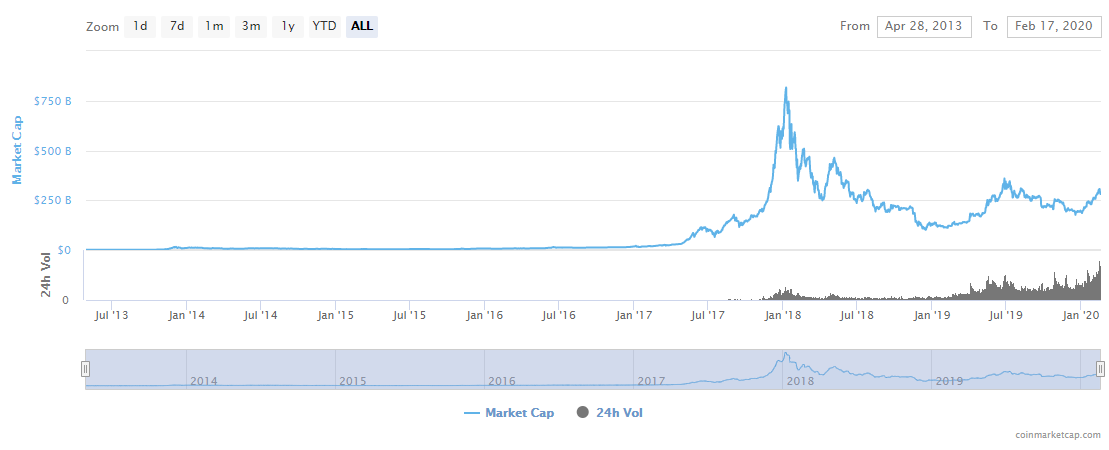
\includegraphics[width=.95\textwidth]{img/ch-iceage/cmc_mcapchart_feb2020.PNG}
    \caption{Global Market Capitalization}
    \label{fig:totalmarketcap}
    \source{Coinmarketcap (17-02-2020); \textit{Global Charts.}}
\end{figure} 

\section{Mondiaal Cryptocurrency Marktperspectief}

Wat wij zeer belangrijk vinden en wat wij specifiek willen benadrukken is dat het noodzakelijk is uit te zoomen om de omvang van deze economie, markt en potentie te begrijpen. Al deze miljarden dollars lijken misschien veel geld, maar laten we al dat geld eens in perspectief plaatsen. \Cref{fig:Cryptocurrency market perspective} geeft je een gevoel van de omvang van deze markt in vergelijking met enkele van de belangrijkste markten wereldwijd.

\begin{figure}[htb]
    \centering
    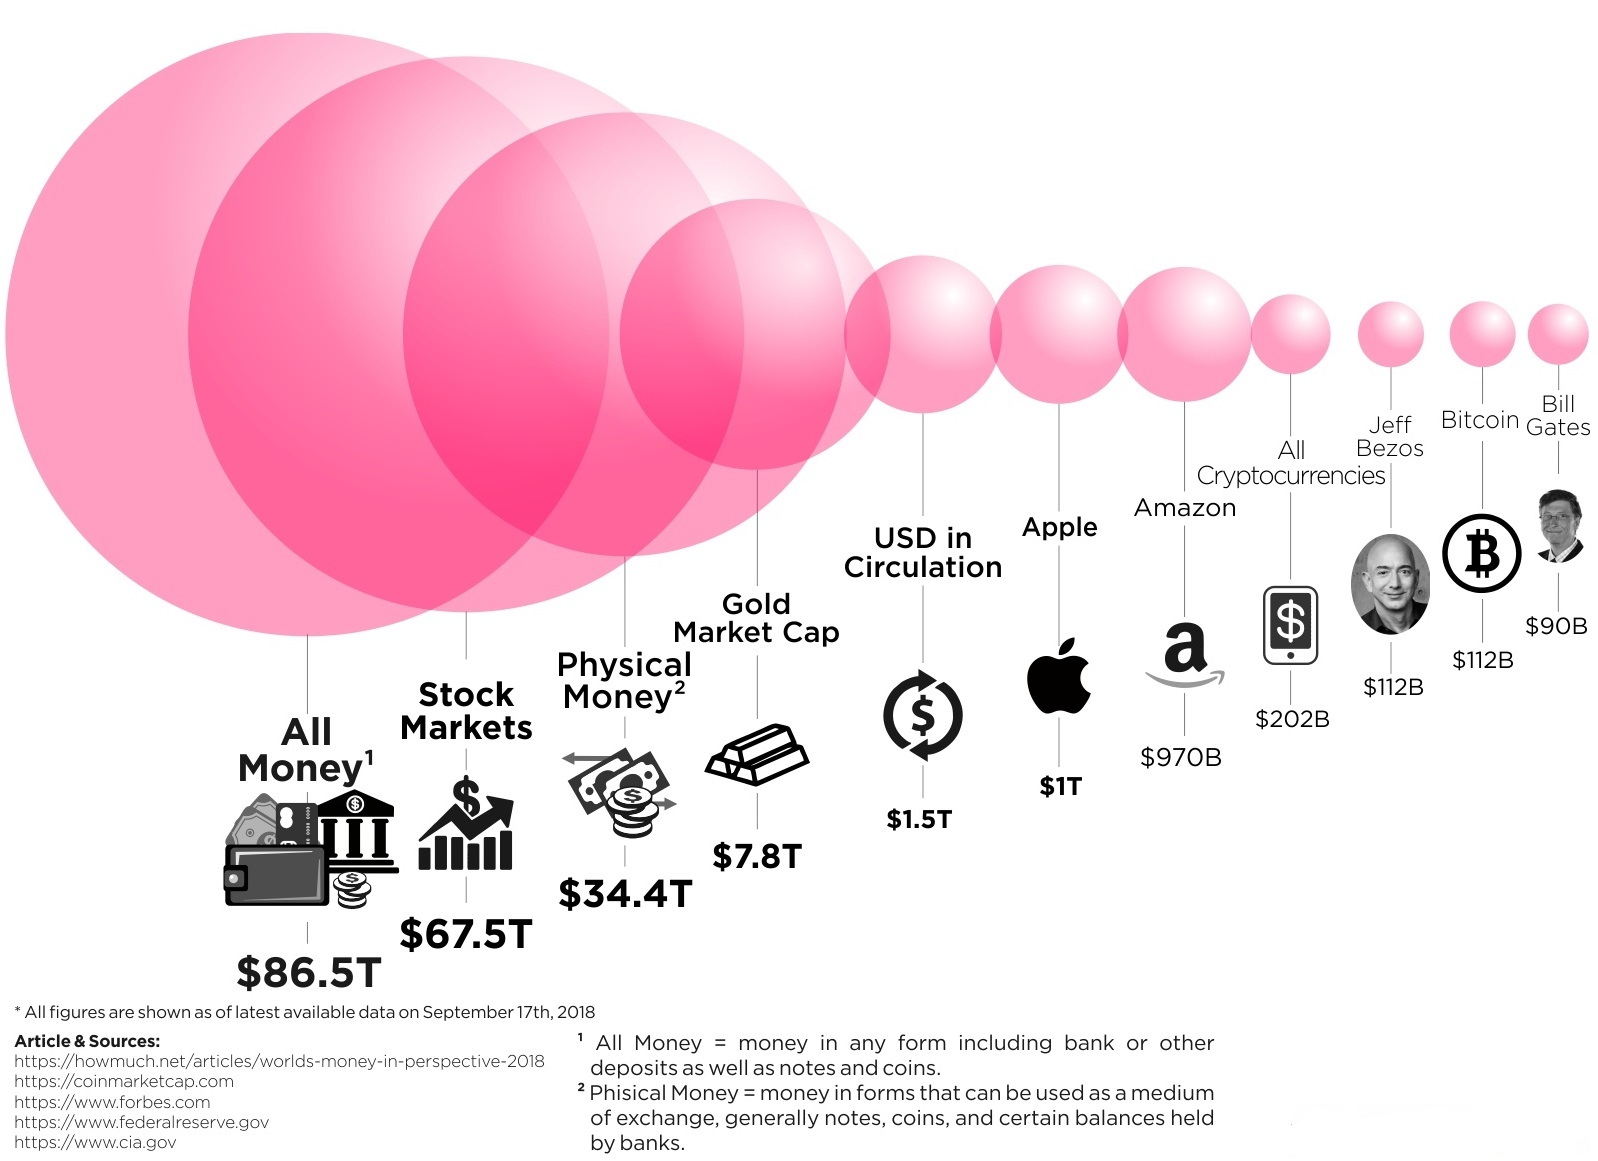
\includegraphics[width=.9\textwidth]{img/ch-iceage/bitcoin-money-economy-in-perspective-2018.jpg}
    \caption{Cryptocurrency Market in Perspective}
    \label{fig:Cryptocurrency market perspective}
    \source{Howmuch, 2018; \textit{Understanding Money.}}
\end{figure}

\noindent Kun je je zelfs een miljard of een biljoen dollar voorstellen? Cryptocurrencies zijn een hot topic; niet alleen tijdens de bubble van eind 2017/begin 2018. Maar zodra de hype voorbij was, keerde de trend om. Door pure paniek verkochten veel mensen hun bezittingen met vreselijke verliezen en zijn nu vastbesloten om nooit meer cryptocurrencies of blockchaintechnologie aan te raken, met het gevoel dat ze beroofd zijn. Aan de andere kant zijn veel mensen die eerder (2013-2017) binnenkwamen misschien juist rijk geworden. Wij richten ons minder op prijs en denken op lange termijn dat deze markt draait om innovatie en verandering, en de kans dat je er gigantische winsten kan opleveren gaan daar vaak gepaard als je investeerd. 

Bovendien gaat het om mensen en projecten die nieuwe technologie gebruiken om ons als mensheid, vooral de mensen in nood, ongelooflijke dingen te brengen. Echter, de meeste mensen in het Westen hebben al toegang tot financiële applicaties, kredieten en het financi\"ele systeem. Zolang niets hun levensstandaard drastisch be\"invloedt, is er geen direct gevoel van urgentie en zeker geen specifieke noodzaak om Bitcoin of enige andere cryptocurrency te leren kennen of zelfs maar te gebruiken.\medskip

Wat dan, over alle mensen in andere gebieden in de wereld die geen gemakkelijke toegang hebben tot financi\"ele diensten zoals bank diensten, reguliere bankrekeningen, mobiele geldtransfers en dergelijke. Noodzaak drijft vaak adoptie, en als er een dringende noodzaak is, ontkiemen de praktijk en de toepassing natuurlijk. Veel landen waar mensen geen toegang hebben tot het financi\"ele systeem maken meer gebruik van nieuwe technologie om toegang te krijgen tot dergelijke diensten. Technologie zoals open blockchain heeft het potentieel om de kwaliteit van het leven van veel mensen over de hele wereld drastisch te be\"invloeden en te verbeteren. \medskip

Hoewel het fantastisch klinkt, hebben veel van deze projecten nog een lange weg te gaan. Wat precies de reden is waarom dit voor ons geen "get-rich-quick-scheme" is, maar een investering voor de lange termijn. Als we kijken naar de omvang van de verschillende wereldmarkten en het stadium van de blockchain en cryptocurrencies op dit moment en de problemen die nog moeten worden opgelost, zal het enige tijd duren voordat deze markt zich kan ontdoen van de volatiliteit en speculatie, liquiditeit problemen, zich kan ontdoen van slechte actoren en zich enigzins kan laten reguleren. Dit alles en nog veel meer is nodig om de weg naar massale adoptie te vergemakkelijken.

\medskip
\tcbset{colback=orange!3!white,fonttitle=\bfseries}
    \begin{tcolorbox}
    [enhanced,
    title=Bull Market 2017/2018,
    frame style=
    {left color=orange!85!black,right color=yellow!95!black}]
    
               \textit{Speculatie en hype waren de dominante marktkrachten tijdens de bull markt in 2017/2018 die in een hyperbubbel eindigde. Bijna alle cryptocurrencies werden overgewaardeerd, en tegelijkertijd was de creatie van reële waarde weinig en ver verwijderd van de werkelijke waarde. Onduurzame en onnatuurlijke groei definieerde deze periode.}
\end{tcolorbox}

\section{Cryptocurrency Markt Vergeleken met de S\&P500}
De derivaten markten houden enorme bedragen (triljoenen) dollars vast en klinken waarschijnlijk onbekend voor velen. Hoe zit het met enkele van de grootste bedrijven ter wereld? Laten we eens kijken naar een aantal van de topbedrijven die genoteerd staan in de S\&P500 (Standard \& Poor's 500 Index). De S\&P500 is een marktkapitalisatie-gewogen index van de 500 grootste Amerikaanse beursgenoteerde ondernemingen naar marktwaarde. De totale waarde van de wereldwijde cryptocurrencymarkt is in januari 2018 vrij dicht in de buurt gekomen van de waarde van een wereldwijd erkende onderneming als Apple of Amazon, maar is sindsdien aanzienlijk gedaald. Deze opkomende markt wordt geplaagd door enorme volatiliteit als gevolg van een gebrek aan investeringen in de markt, lage liquiditeit en echte fundamentele gebruiksdoelen.
Toch zijn er, zoals eerder aangegeven, bijna 4000 projecten of cryptokringen die elk hun eigen en unieke doelstellingen en ambities hebben. Sommige (niet alle) projecten maken gebruik van revolutionaire nieuwe technologi\"en en kunnen op de lange termijn zeer verstorend zijn voor bestaande markten (en dus voor bedrijven!). Het is mogelijk dat uit de huidige 4000 projecten - met ondernemers over de hele wereld die bijna dagelijks nieuwe projecten lanceren - verschillende bedrijven van de volgende generatie zullen ontstaan.\medskip 

Hoewel de cryptocurrency markt overeenkomsten kan hebben met grote bedrijven in termen van marktaandeel, is het punt dat veel cryptocurrency projecten fundamenteel verschillend zijn van reguliere bedrijven of bedrijven in de manier waarop ze werken en functioneren. We verwachten op zijn minst een aantal successen waar blockchainprojecten een aanzienlijke verstorende invloed zouden kunnen hebben. Op de lange termijn zal dit leiden tot een toename van het marktaandeel, dat wordt gedreven door de revolutionaire nieuwe fundamenten en bedrijfsmodellen van deze nieuwe bedrijven.

\section{Alternatieve Cryptocurrencies (Altcoins)}
Bitcoin domineerde de cryptocurrency markt volledig tot de altcoin en ICO boom in 2017.  \say{altcoin} is een combinatie van twee woorden: \say{alt} en \say{coin}; alt staat voor \say{alternatieve} en coin staat voor Bitcoin of \say{cryptocurrency}. Samen impliceren ze een categorie van cryptocurrencies die een alternatief is voor de cryptocurrency Bitcoin. Na het succes van de Bitcoin zijn veel andere peer-to-peer digitale cryptocurrencies ontstaan in een poging om dat succes te imiteren of de technologie verder te evolueren. 

\medskip
\tcbset{colback=orange!3!white,fonttitle=\bfseries}
    \begin{tcolorbox}
    [enhanced,
    title=Altcoins,
    frame style=
    {left color=orange!85!black,right color=yellow!95!black}]
       \textit{Terwijl Bitcoin de eerste cryptocurrency was, en de enige cryptocurrency die op de grootste schaal is getest zonder enige significante mislukking, is het nu slechts \'e\'en van de meer dan duizend cryptocurrencies, die allemaal proberen de Bitcoin te verbeteren of te innoveren, techniek te revolutioneren en bestaande markten te ontwrichten in verschillende andere segmenten..}
\end{tcolorbox}
\medskip

Veel van deze altcoins hebben gebouwd op de noodzakelijke raamwerken van Bitcoin of hebben hun eigen blokchain architectuur ontwikkeld. Vanwege de gedecentraliseerde en gedistribueerde architectuur van de meeste blockchainnnetwerken zijn de meeste altcoins peer-to-peer, bevatten ze een mining proces waarbij gebruikers ernstige problemen oplossen om blokken te ontsluiten en bieden ze effici\"ente en goedkope manieren om (waarde)transacties op het web uit te voeren. Echter, zelfs met veel overlappende functies, verschillen altcoins sterk van elkaar - altcoins verschillen zelf van Bitcoin met een scala aan procedurele variaties, waaronder verschillende consensusalgoritmes, transactiesnelheden en schaalbaarheidsniveaus. Ze zetten ook verschillende middelen in waarmee gebruikers blokken kunnen minen, beloond worden en ze maken gebruik van applicatieverbeteringen om bijvoorbeeld de anonimiteit van de gebruiker te vergroten. Zoals gezegd zijn er op dit moment enorm veel cryptocurrencies, en dat aantal groeit nog steeds. Het uitvoeren van fundamentele analyses op altcoins is een must voordat je beslissingen neemt. Daarvoor zijn de basisprincipes uiteengezet in de sectie over het doen van je eigen onderzoek  (\cref{ch:research}). Sinds de altcoin-explosie in 2017 is de dominantie van de Bitcoin aanzienlijk afgenomen door steeds meer veelbelovende projecten met verschillende usecases en niches te vervullen.

\begin{figure}
    \centering
    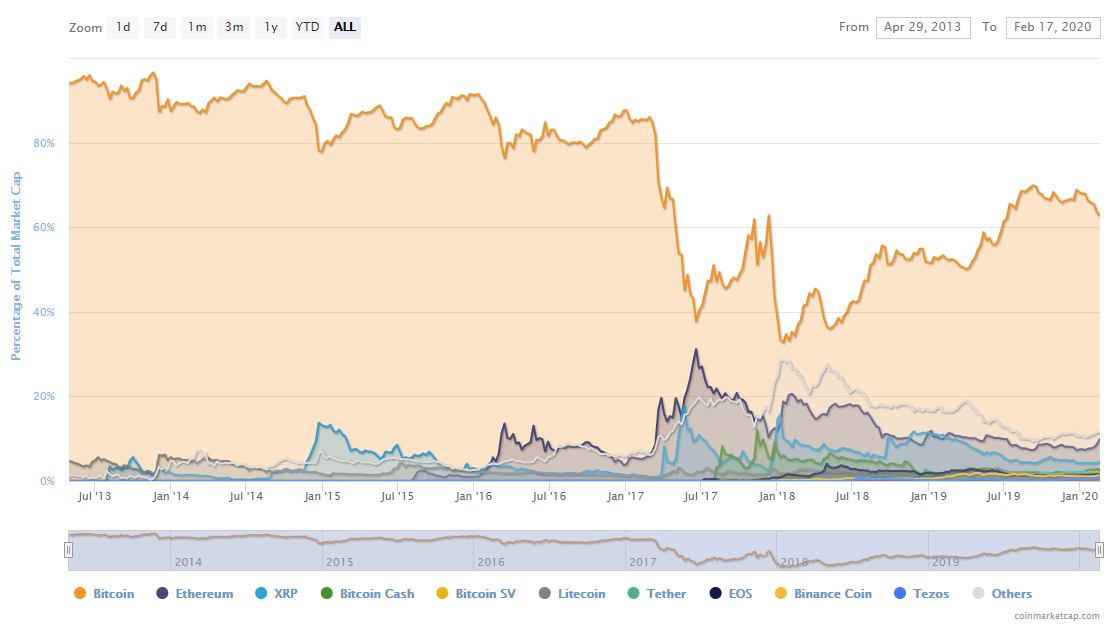
\includegraphics[width=.95\textwidth]{img/ch-iceage/cmc_domchart_feb2020.PNG}
    \caption{Percentage of Global Market Cap (Dominance)}
    \label{fig:Total market capitalization dominance}
    \source{Coinmarketcap (17-02-2020); \textit{Global Charts.}}
\end{figure} 

\section{Initial Coin Offerings (ICOs)}
Het is ongelooflijk om te beseffen hoeveel de altcoinmarkt alleen al in de afgelopen vier jaar is gegroeid. ICO's zijn zo populair geworden dat meer dan 90\% van de totale investeringen die via dit mechanisme zijn opgehaald, alleen al uit 2018 komen. Hoewel het moeilijk is om deze plotselinge ICO-explosie in de context te plaatsen, zijn er animaties en info-grafhics \footnote{Elementus (39-09-2018); \href{https://elementus.io/blog/ico-market-august-2018}{ICO Market August 2018}.}\footnote{Visual Capitalist (30-12-2017); \href{https://www.visualcapitalist.com/the-rise-of-the-ico}{The Rise of the ICO}.} die het fenomeen voldoende recht doen en die een tijdlijn laten zien van de ICO's en de investeringen die sinds begin 2014 zijn opgehaald. 

\subsection{ICO Scams}

Er is een groot verschil tussen een typische ICO nu en \'e\'en in 2017. Een duizelingwekkende hoeveelheid ICO's heeft het niet eens gehaald tot een exchange - volgens een studie uitgevoerd op de kwaliteit van ICO's door  Statis\footnote{Medium (25-05-2018); \href{https://medium.com/satis-group/ico-quality-development-trading-e4fef28df04f}{ICO quality: Development \& Trading}.}. Het grootste deel van het geld wordt nu opgehaald via particuliere aanbiedingen, terwijl openbare verkoop zeldzaam is geworden. Waarom? Het is geen goed beeld voor de markt om retailbeleggers te laten doen geloven dat ze kunnen profiteren van voorstellen met een hoge inzet die hen een hoop geld kunnen doen verliezen. Ze beloven grote bergen goud, maar moeten nog maar zien of ze de torenhoge beloftes kunnen inlossen.

Houd er rekening mee dat het altijd mogelijk is dat een project of een coin een oplichterij is en wees sceptisch bij het beoordelen of het kan waarmaken wat het heeft beloofd . Mensen kunnen hun vertrouwen verliezen, ontwikkelaars kunnen slechte bedoelingen hebben of het project opgeven. Het reguleringsbeleid en de nalevingskaders waren in 2017 nog niet eens in de buurt van de invoering ervan (veel instellingen worden buitenspel gezet), maar het reguleringslandschap evolueert snel. Deze factoren zouden wel eens het einde van je investering kunnen betekenen als je op het hoogtepunt van de bubbel hebt ge\"investeerd terwijl de prijzen kelderden en de ontwikkeling tot stilstand kwam. Je kunt controleren of een munt of project wordt gerapporteerd als een oplichterij of een dode munt op Coinopsy\footnote{Coinopsy (05-02-2019);
\href{https://www.coinopsy.com/dead-coins}{Dead Coins}.} and on Deadcoins\footnote{Deadcoins (05-02-2019); \href{https://deadcoins.com}{Full List of Dead Coins}.}. Dit verhaal heeft nauwe banden met onze afdeling over hoe u uw onderzoek (\cref{ch:research}) kunt uitvoeren en voorkomt dat je wordt opgelicht. 

